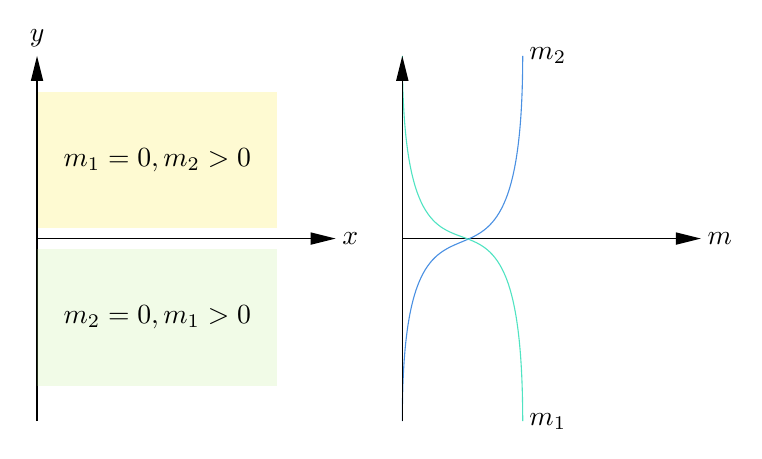
\begin{tikzpicture}[x=0.75pt,y=0.75pt,yscale=-1,xscale=1]
    %uncomment if require: \path (0,300); %set diagram left start at 0, and has height of 300
    
    %Shape: Rectangle [id:dp1437775685732261] 
    \draw  [draw opacity=0][fill={rgb, 255:red, 248; green, 231; blue, 28 }  ,fill opacity=0.2 ] (100,53.38) -- (215.83,53.38) -- (215.83,119.19) -- (100,119.19) -- cycle ;
    %Straight Lines [id:da2865557283068807] 
    \draw    (100,212.19) -- (100,38.19) ;
    \draw [shift={(100,36.19)}, rotate = 90] [fill={rgb, 255:red, 0; green, 0; blue, 0 }  ][line width=0.08]  [draw opacity=0] (12,-3) -- (0,0) -- (12,3) -- cycle    ;
    %Straight Lines [id:da6631589276488061] 
    \draw    (100,124.19) -- (241.83,124.19) ;
    \draw [shift={(243.83,124.19)}, rotate = 180] [fill={rgb, 255:red, 0; green, 0; blue, 0 }  ][line width=0.08]  [draw opacity=0] (12,-3) -- (0,0) -- (12,3) -- cycle    ;
    %Shape: Rectangle [id:dp34779645053953057] 
    \draw  [draw opacity=0][fill={rgb, 255:red, 184; green, 233; blue, 134 }  ,fill opacity=0.2 ] (100,129.19) -- (215.83,129.19) -- (215.83,195) -- (100,195) -- cycle ;
    %Straight Lines [id:da6534837649049938] 
    \draw    (276,124.19) -- (417.83,124.19) ;
    \draw [shift={(419.83,124.19)}, rotate = 180] [fill={rgb, 255:red, 0; green, 0; blue, 0 }  ][line width=0.08]  [draw opacity=0] (12,-3) -- (0,0) -- (12,3) -- cycle    ;
    %Curve Lines [id:da9931229569829934] 
    \draw [color={rgb, 255:red, 74; green, 144; blue, 226 }  ,draw opacity=1 ]   (276,212.19) .. controls (275.83,62.19) and (333.83,190.19) .. (334,36.19) ;
    %Curve Lines [id:da29237588773234124] 
    \draw [color={rgb, 255:red, 80; green, 227; blue, 194 }  ,draw opacity=1 ]   (334,212.19) .. controls (333.83,56.19) and (276.17,190.19) .. (276,36.19) ;
    %Straight Lines [id:da5969937344693497] 
    \draw    (276,212.19) -- (276,38.19) ;
    \draw [shift={(276,36.19)}, rotate = 90] [fill={rgb, 255:red, 0; green, 0; blue, 0 }  ][line width=0.08]  [draw opacity=0] (12,-3) -- (0,0) -- (12,3) -- cycle    ;
    
    % Text Node
    \draw (100,33.19) node [anchor=south] [inner sep=0.75pt]    {$y$};
    % Text Node
    \draw (157.92,86.28) node    {$m_{1} =0,m_{2}  >0$};
    % Text Node
    \draw (157.92,162.09) node    {$m_{2} =0,m_{1}  >0$};
    % Text Node
    \draw (245.83,124.19) node [anchor=west] [inner sep=0.75pt]    {$x$};
    % Text Node
    \draw (421.83,124.19) node [anchor=west] [inner sep=0.75pt]    {$m$};
    % Text Node
    \draw (336,36.19) node [anchor=west] [inner sep=0.75pt]    {$m_{2}$};
    % Text Node
    \draw (336,212.19) node [anchor=west] [inner sep=0.75pt]    {$m_{1}$};
    
    
    \end{tikzpicture}
    